% Documentatie Herfstkamp project: Bouw van een audio-versterker
% Jules Hammenecker
% Vrije Universiteit Brussel - Dept. ELEC
% Augustus 2015

\title{Project Ingenieurswetenschappen: \\ Elektronisch ontwerp van de e-VUBOX~speaker\\ Labonota's}
\author{Vrije Universiteit Brussel}
\date{Versie 08.2015}

\documentclass{article}
	\usepackage[a4paper]{geometry}
	%\usepackage[utf8x]{inpudetenc}
	\usepackage[T1]{fontenc}
	\usepackage[dutch]{babel}
	\usepackage{amsmath}

	\newtheorem{DIY}{Doe-het-zelf}
	\usepackage{multicol}
	%%% FIGURES %%%
	\usepackage[pdftex]{graphicx}
	\usepackage{caption,subcaption}
	\usepackage{hyperref}
	\graphicspath{ {./figs/} }

\begin{document}
	
	\maketitle

	\tableofcontents
	\clearpage

\section{Basis Elektronica}

			\begin{DIY} Wat is de waarde $R$ van een weerstand waarover een spanning van $V = 25~V$ is en waardoor een stroom van $I = 0.1~A$ loopt?
			\begin{align}
			    R = \ldots
			\end{align}
			\end{DIY}
		\vspace{20ex}

			\begin{DIY} Pas de stroomwet van Kirchhoff toe in figuur \ref{subfig:kcl_oef}, en vind de missende stromen. Doe hetzelfde voor de spanningen in figuur \ref{subfig:kvl_oef}.
			\begin{align*}
			    I_1 &= \ldots \\
			    V_1 &= \ldots 
			\end{align*}
			\end{DIY}

			\begin{figure}[htbp]
				\centering
				\begin{subfigure}[b]{0.45\linewidth}
					\centering
					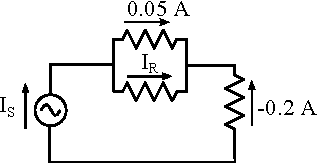
\includegraphics[width=0.7\textwidth]{kcl_oef.pdf}
					\caption{Vind $I_R$ en $I_s$.}
					\label{subfig:kcl_oef}
				\end{subfigure}
				~
				\begin{subfigure}[b]{0.45\linewidth}
					\centering
					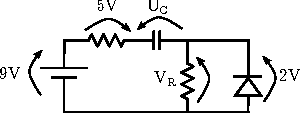
\includegraphics[width=0.9\textwidth]{kvl_oef.pdf}
					\caption{Vind $V_R$ en $U_C$. }
					\label{subfig:kvl_oef}
				\end{subfigure}
			\caption{De wetten van Kirchhoff}
			\label{fig:kirchoff_oef}
			\end{figure}
\vspace{40ex}
\section{Bouwstenen van de e-VUBOX}
		\subsection{De volumeknop: de spanningsdeler}

			\begin{figure}[htbp]
				\centering
				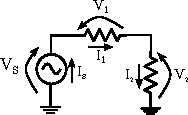
\includegraphics[width=0.3\textwidth]{weerstandsdeler}
				\caption{Volumeregeling: de spanningsdeler}
				\label{fig:volume}
			\end{figure}

			Wetten van Kirchhoff:
			\begin{align}
			    I_S &= I_1 = I_2 \\
			    V_S &- V_1 -V_2 = 0 
			\end{align}
			Wet van Ohm:
			\begin{align}
			    V_1 = R_1 \cdot I_1 \\
			    V_2 = R_2 \cdot I_2
			\end{align}

			\begin{DIY} Vind nu, dankzij de vier vorige vergelijkingen, de uitdrukking voor de spanning $V_2$ in functie van $V_s$, $R_1$ en $R_2$. Omdat we alleen de spanningsverhouding willen weten, mogen er geen stromen voorkomen in de formule.
			\begin{align*}
			    V_2 = \ldots\ldots
			\end{align*}
			\end{DIY}
\vspace{40ex}
			\begin{DIY} Je heb een voltage van $9$ V als ingangsspanning $V_S$, en je wilt een voltage van $1.5$ V als uitgangsspanning $V_2$. $R_1$ is al gekozen en heeft een weerstand van $1$ k$\Omega$ ($1000 \Omega$). Welke waarde moet je kiezen voor $R_2$?
			\begin{align*}
			    R_2 = \ldots\ldots
			\end{align*}
			\end{DIY}
\vspace{50ex}
			\begin{DIY} Welke weerstand $R_{pot}$ moet de potentiometer hebben, wetend dat de ingangsspanning $V$ maximaal $200$ mV ( = $200 \cdot 10^{-3}$ V)is en we het vermogen $P$ willen beperken tot 4 $\mu$W ( = $4 \cdot 10^{-6}$ W)? \textbf{Tip:} De formule voor elektrisch vermogen kan je vinden op pagina \pageref{eq:vermogen},  je hebt de wet van Ohm ook nodig.
			\begin{align*}
			    R_{pot} = \ldots\ldots
			\end{align*}
			\end{DIY}			

\vspace{30ex}
		\subsection{Het statusledje: de diode}
			

				\begin{figure}[htbp]
					\centering
					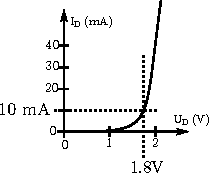
\includegraphics[width=0.5\textwidth]{diode_grafiek}
					\caption{Grafiek van de stroom in functie van de spanning van een diode.}
					\label{fig:diode_grafiek}
				\end{figure}


			\begin{figure}[htbp]
				\centering
				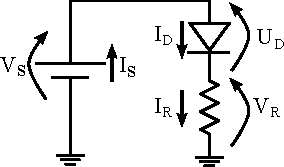
\includegraphics[width=0.3\textwidth]{diode_netwerk}
				\caption{Diode netwerk.}
				\label{fig:diode_netwerk}
			\end{figure}

			\begin{align}
				+V_s &- U_D - V_R = 0  \\
				I_s &= I_D = I_R
			\end{align}

			\begin{DIY} Kan je de waarde vinden van de weerstand die nodig is? \textbf{Tip:} bepaal $I_R$ en $V_R$ uit de wetten van Kirchhoff.
			\begin{align*}
			    R_{led} = \ldots\ldots
			\end{align*}
			\end{DIY}
\vspace{30ex}

		\subsection{De versterker: de transistor}
			
			\subsubsection{De bipolaire npn transistor}
				\begin{figure}[htbp]
				\centering
					\begin{subfigure}[b]{0.45\linewidth}
						\centering
					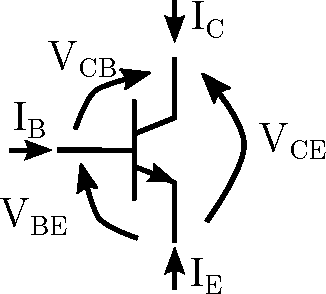
\includegraphics[width=0.7\textwidth]{transistor_VI}
					\caption{Schematische voorstelling van de bipolaire transistor met stromen en spanningen. Alle stromen worden conventioneel \textbf{naar} de transistor toe getekend.}
					\label{subfig:transistor_vi}
					\end{subfigure}
					~
					\begin{subfigure}[b]{0.45\linewidth}
						\centering
						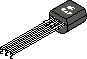
\includegraphics[width=0.6\textwidth]{transistor}
						\caption{De BC547 bipolaire transistor met Basis, Collector en Emitter aangeduid.}
						\label{subfig:transistor_bce}
					\end{subfigure}
					
					\caption{De bipolaire npn transistor.}
					\label{fig:transistor}
				\end{figure}

				De regels waaraan een bipolaire transistor zich moet houden zijn:
				\begin{enumerate}
\item
					\begin{align}
					    V_{CB} > 0~V. 
					\end{align}

\item
					\begin{align}
					    V_{BE} \approx 0.7~V
					\end{align}

					\item $I_C, I_B$ en $V_{CE} $ moeten binnen bepaalde maximale waarden liggen.

					\item Als aan de drie vorige regels is voldaan, dan is de collectorsstroom een versterkte versie van de basisstroom: 
					\begin{align}
					    I_C = \beta I_B
					    \label{eq:hfe}
					\end{align}
					$\beta$ (ook als $h_{FE}$ genoteerd) wordt de stroomversterkingsfactor genoemd.

				\end{enumerate}

				De wetten van Kirchhoff gelden ook voor de transistor:
				\begin{align}
				    I_C		&+ I_B = -I_E \\
				    V_{BE}  &+ V_{CB} - V_{CE} = 0
				\end{align}

				\begin{DIY} Elimineer $I_B$ van de stroomwet van Kirchhoff met behulp van vergelijking (\ref{eq:hfe}). Vind dan een uitdrukking voor $I_C$. Stel dan dat $\beta = 250$, en rond af. Welke relatie vind je tussen $I_C$ en $I_E$? 
				\begin{align*}
				    I_C \approx \ldots \ldots
				\end{align*}
				\end{DIY}
\vspace{30ex}
			\subsubsection{Het versterkingsnetwerk}


				\begin{figure}[htbp]
					\centering
					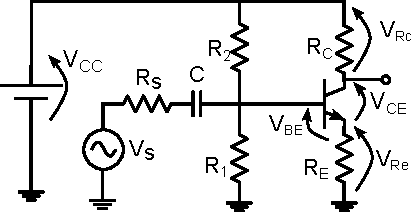
\includegraphics[width=0.8\textwidth]{ges}
					\caption{Versterkerschakeling met de transistor.}
					\label{fig:ges}
				\end{figure}

				$R_s$ is de serieweerstand van de spanningsbron, en $C$ is een ontkoppelcapaciteit.
		
				Om de versterker te ontwerpen moeten we de weerstanden $R_1,R_2,R_E$ en $R_C$ kiezen.

				\begin{DIY} Vind een uitdrukking voor de spanning aan de collector $V_C$ in functie van de basisspanning $V_B$, en vind dat je de spanning $V_B$ versterkt. We hebben volgende vergelijkingen die we kunnen gebruiken:
				\begin{itemize}
					\item de spanningswet van Kirchoff
					\begin{align}
					V_{Re} + V_{CE} + V_{Rc} - V_{CC} = 0    
					\end{align}
					\item de transistorvergelijkingen\footnote{ $V_{BE}$  is de spanning tussen B en E, $V_{B}$ is de spanning tussen B en de grond (hetzelfde voor $V_C$ en $V_E$). We kunnen dan schrijven dat $ V_{BE} = V_{B} - V_{E} $}
					\begin{align}
				    V_{BE} &= V_{B} - V_{E} = 0.7~V \\
				     I_C&\approx -I_E \\
				    V_{CE} &= V_C - V_E > 0
					\end{align}
					\item de weerstandsvergelijkingen
					\begin{align}
				   	V_{Rc} &= R_C \cdot I_C \\
				   	V_{Re} &= - R_E \cdot  I_E
					\end{align}
					De wet van Ohm geldt als de spanning- en stroomrichting tegengesteld zijn. Indien ze in dezelfde richting zijn, komt er een minteken in de wet.
				\end{itemize}

				\textbf{Tip:} \'e\'en manier om het te vinden: druk de stroom uit door $R_C$ met de wet van Ohm. Die is nodig om de spanning $V_E$ te vinden die je dan gebruikt om $V_B$ te vinden. Vorm de vergelijking dan om om $V_C$ te isoleren.
				\begin{align}
				    V_C = \ldots \ldots \ldots \ldots  \ldots  \ldots 
				\end{align}
\vspace{30ex}
				\end{DIY}



				De methode gaat als volgt:
				\begin{enumerate}
					\item Kies de gemiddelde stroom $I_C$.
					\begin{align}
					    I_C = \ldots
					\end{align}

					\item Kies een gemiddelde voltage $V_C$, waar de muziekgolf rond gaat vari\"eren.
					\begin{align}
					    V_C = \ldots
					\end{align}


					\item Laatste keuze: kies een versterkingsfactor $- \frac{R_C}{R_E}$.
					\begin{align}
					    -\frac{R_C}{R_E} = \ldots
					\end{align}
				\end{enumerate}


				\begin{DIY} Je kent nu alles wat nodig is om de weerstanden $R_{E}$ en $ R_{C}$ te bepalen. \textbf{Tip:} Uit $I_C$ en $V_C$ kan je de waarde $R_C$ vinden.
				\begin{align}
				    R_C &= \ldots \\
				    R_E &= \ldots
				\end{align}
\vspace{30ex}
				\end{DIY}				


				\begin{DIY} Bereken het biasvoltage $V_B$. Kies dan de weerstand $R_2$ zodat $V_B$ de gewenste waarde heeft. Het staat al vast dat $R_1 = 1k\Omega$. \textbf{Tip:} Herinner U dat $V_{CC} = 9V$ en de formule van de weerstandsdeler.
				\begin{align}
				    R_1 &= 1k\Omega \\
				    R_2 &= \ldots
				\end{align}
\vspace{50ex}
				\end{DIY}


				\begin{center}
					\noindent \fbox{ 
						\parbox{0.8\textwidth}{
							Samenvatting van de gekozen weerstanden:
							\begin{align*}
							    R_1 &= \ldots \\
							    R_2 &= \ldots \\
							    R_E &= \ldots \\
							    R_C &= \ldots
							\end{align*}
						}
					 }
				\end{center}


	\section{Conclusie}

		\begin{figure}[htbp]
			%\centering
			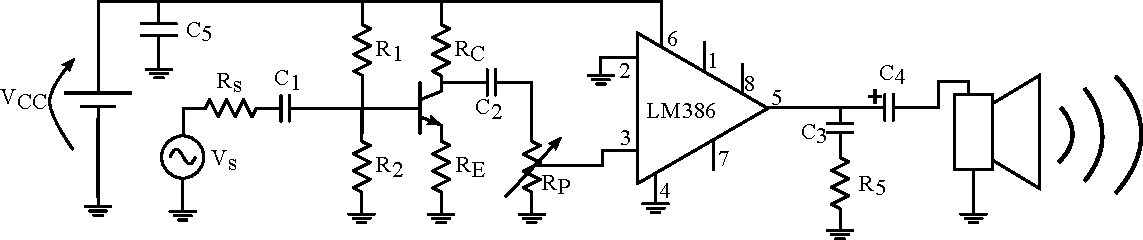
\includegraphics[width=\linewidth]{volledig_schema}
			\caption{Volledig Schema}
			\label{fig:volledig_schema}
		\end{figure}
		$C_1$ en $C_2$ zijn ontkoppelcapaciteiten dienen om DC signalen te blokkeren, $C_5$ werkt als een hulpbatterij.
		\begin{center}
			\noindent \fbox{ 
				\parbox{0.8\textwidth}{
					\begin{align*}
						R_1 &= 1~k\Omega & R_2 &= 4.7~k\Omega \\
						R_E &= 100~\Omega & R_C &= 560~\Omega \\
						R_P &= 10~k\Omega & R_5 &= 10~\Omega \\
						R_{LED} &= 680~\Omega
					\end{align*}
				}
			 }
		\end{center}

		De waardes van de capaciteiten zijn:
		\begin{center}
			 			\noindent \fbox{ 
				\parbox{0.8\textwidth}{
					\begin{align*}
						C_1 &= 1~\mu F & C_2 &= 42 ~\mu F \\
						C_3 &= 100~nF & C_4 &= 220~ \mu F \\
						C_5 &= 330~\mu F
					\end{align*}
				}
			 }
		\end{center}
\end{document}